\documentclass[10pt]{article}
\usepackage{float}
\RequirePackage{eso-pic}
\usepackage{caption}
\captionsetup[table]{labelformat=empty}



\usepackage{geometry}
\geometry{
a4paper,
left=11mm,
right=14mm,
top=37mm,
bottom=14mm,
}



\usepackage{colortbl}
\usepackage{fontspec}
\setmainfont[Ligatures=TeX]{Calibri}



\newcommand\BackgroundPic{%
\put(0,0){%
\parbox[b][\paperheight]{\paperwidth}{%
\vfill
\centering
\includegraphics{MBIE_generic_background.pdf}%
\vfill
}}}



\begin{document}
\thispagestyle{empty}
\AddToShipoutPicture{\BackgroundPic}
\section*{Key Export Statistics\footnotemark - Biscuits\footnotemark }
Published on April 07, 2016. \par
\small{\noindent{\textit{Monthly data from January 2000 to November 2015.}}}
\begin{table}[ht]
\centering
{\scriptsize
\begin{tabular}[t]{p{1.8cm}>{\hfill}p{1.4cm}>{\hfill}p{1.4cm}>{\hfill}p{1.6cm}>{\hfill}p{1.9cm}>{\hfill}p{2cm}>{\hfill}p{1.9cm}>{\hfill}p{1.5cm}}
 \textbf{Country} & \textbf{Yearly Qty} & \textbf{Yearly Value} & \textbf{Yearly Price} & \textbf{3Year CAGR(Qty)} & \textbf{3Year CAGR(Value)} & \textbf{3Year CAGR(Price)} & \textbf{Price Elasticity} \\
\hline
Australia & 5,024 & 35.3 & \$7.0 & 5.6\% & 2.8\% & -2.6\% & -2.2 \\  
China & 170 & 2.4 & \$13.9 & 29.7\% & 65\% & 27.2\% & 1.1 \\  
Hong Kong & 67 & 1.1 & \$16.7 & 62\% & 81.9\% & 12.3\% & 5.1 \\  
Malaysia & 230 & 0.8 & \$3.7 & 8.1\% & 7.9\% & -0.2\% & -47.2 \\  
New Caledonia & 109 & 0.8 & \$7.4 & 14.9\% & 15.2\% & 0.2\% & 79.9 \\  
Singapore & 106 & 0.5 & \$4.9 & 114.1\% & 76.6\% & -17.5\% & -6.5 \\  
Other & 334 & 2.3 & \$6.8 & 5.4\% & 5.9\% & 0.5\% & 11.0 \\  
Total & 6,040 & 43.2 & \$7.2 & 7.1\% & 5.9\% & -1.1\% & -6.4 \\  
\hline
\end{tabular}
}
\caption{\scriptsize Top 6 Biscuits Markets for year ending November - 2015: Quantity('000 kg) Value(NZ\$Mill), Price and their last 3-Year Growth Rates}
\end{table}


\vspace{-0.7cm}



   \begin{figure}[H]
   \centering
    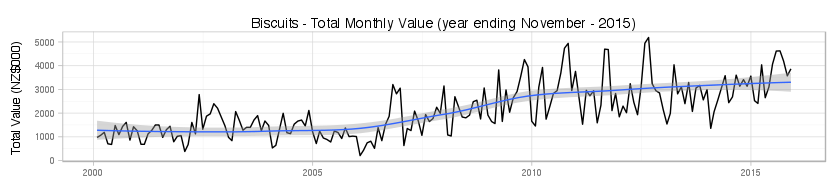
\includegraphics[scale=0.5]{../graphs/monthly_value/biscuits_monthly_value.png} \
    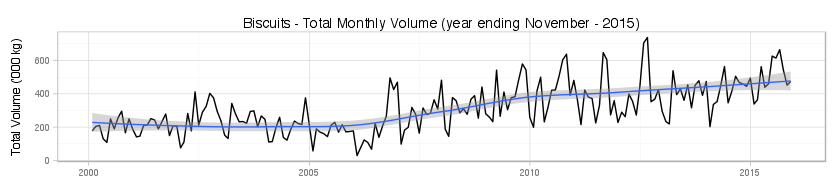
\includegraphics[scale=0.5]{../graphs/monthly_volume/biscuits_monthly_volume.png} \
    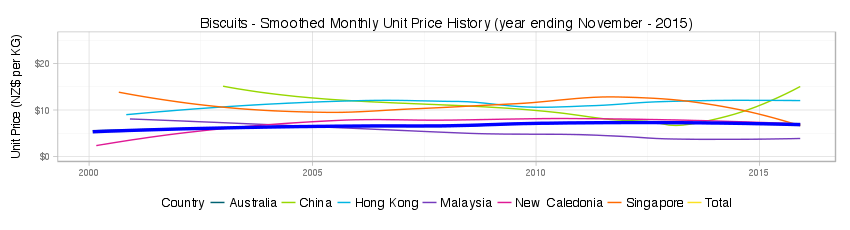
\includegraphics[scale=0.5]{../graphs/smoothed_price/biscuits_smoothed_price.png} \
    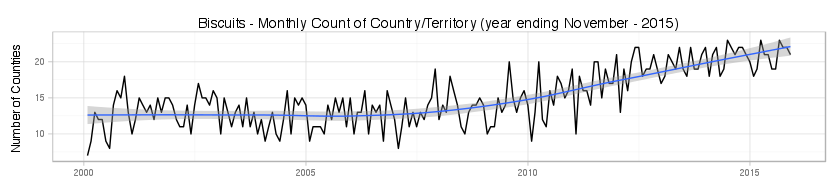
\includegraphics[scale=0.5]{../graphs/monthly_number_countries/biscuits_monthly_count.png} \
    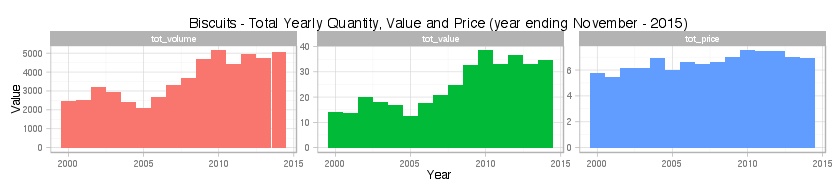
\includegraphics[scale=0.5]{../graphs/yearly_summary/biscuits_yearly_summary.png} \
   \end{figure}



\footnotetext[1]{Source: Statistics New Zealand - Overseas Merchandise Trade}
\footnotetext[2]{Harmonised System Codes for Biscuits starting with: 190530, 190531, 190590.}
\end{document}
